\documentclass{bhamthesis}
\title{Solving Match Three with Artificial Intelligence: A Comparison of Evaluation Functions}
\author{Thomas Brereton}
\date{August 2017}  %% Version 2009/12/26

\usepackage{amsthm}
\usepackage{amssymb}
\usepackage{graphicx}
\usepackage{blindtext}
\usepackage[toc]{glossaries}


\usepackage[backend=biber]{biblatex}
\addbibresource{references.bib}


\newtheorem*{thm}{Theorem}

\theoremstyle{definition}
\newtheorem*{defn}{Definition}

\newcommand{\mar}[1]{\marginpar{\raggedright#1}}
\newcommand{\clsname}{\textsf{bhamthesis}}
\newcommand{\bktitle}[1]{\textit{#1}}
\newcommand{\ZF}{\mathrm{ZF}}
\newcommand{\IN}{\mathbb{N}}

\makeatletter
\newcommand{\makecrestcover}{%
\begin{titlepage}
\centering\singlespacing
\vspace*{1cm}
{\huge\bfseries University of Birmingham\par}
\vspace*{2cm}

\includegraphics[width=.3\textwidth]{crest}\par
\vspace*{\stretch{1}}
{\Huge\bfseries
\@author\par
\vspace{1cm}
\@title\par}
\vspace*{\stretch{1}}
{\Large\@date\par}
\end{titlepage}
}
%\makeatother
%
%\prefixappendix


\makeglossaries

\newglossaryentry{latex}
{
	name=latex,
	description={Is a mark up language specially suited 
		for scientific documents}
}


\begin{document}
\frontmatter

%% Optional/alternative cover with crest
%\makecrestcover
\maketitle


\begin{abstract}
To be completed.
\end{abstract}

\tableofcontents
\mainmatter

\chapter{Introduction}
The game of Go has long been considered the hardest challenge of artificial intelligence (AI) due to its intractable search space (approx. $10^{170}$ possible states \cite{Gelly2012}). However, the game of Go is still deterministic in the sense that if we are in state $s_0$, and select a legal action $a_0$, we must transition to $s_1$, given the opponent is rational. This is far from real-life scenarios where there is significant factors of hidden information and randomness. This motivated us to build an AI program which would perform successfully in partially observable Markov Decision Processes (POMDPs) with stochastic elements. In this report we use Monte Carlo Tree Search (MCTS) and neural networks (NN) to beat a POMDP game (with stochastic elements) of our own making, Gem Island. 

The aim of Gem Island (refer Section \ref{s:gamed}) is to match three or more gems of the same type over the ice to free the medals underneath. Each game begins by generating gems in a nine by nine grid each of which is randomly one of six different types. Additionally, opaque ice covers the bottom five row of the game to hide the medals, which are randomly placed underneath. Figure \ref{f:gemIsland} illustrates a beginning state of the game. A legal move is made by swapping two adjacent gems which results in at least one match.

\begin{figure}[h]
	\centering
	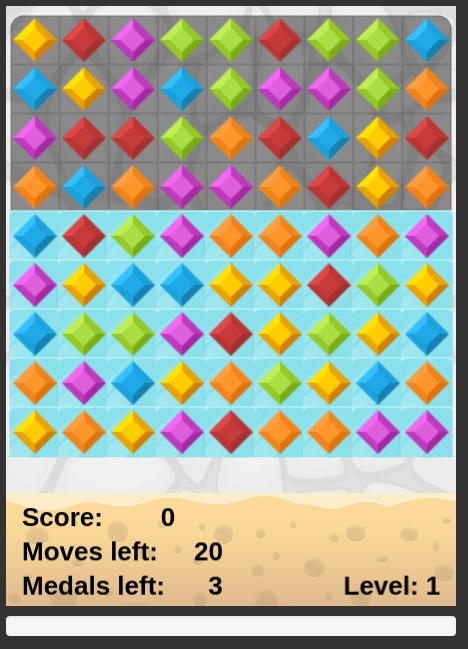
\includegraphics[width=0.4\textwidth]{media/img/screen2}
	\caption{Gem Island: a match three game.}\label{f:gemIsland}
\end{figure}

To account for the hidden information of the medals, we used a simulator to predict state $s$ given observations $o$. To handle the stochastic elements of the gem generation we used a flat UCT MCTS \cite{Browne2012}, which stores the actions only from the root state rather than building a tree. 

The main contribution of this report is the comparison of different MCTS programs with varying evaluation functions. We find that the Heuristic Based (HB) evaluation function (refer Section \ref{s:hbF}) performs best with a win rate of 87\% and mean moves made of 12.5. in comparison to human ability, this is better than average (43\%) and comparable to elite human play (89\%).

The second contribution is the game of Gem Island. It provides a standard test bed for POMDPs with stochastic elements and it is designed with an application programming interface (API) suited for AI research, including a method for gathering data, easy access to the game state, and a simple method of connecting AI controllers. Gem Island has a much larger branching factor than full sized Go and its search space is also larger than $9 \times 9$ Go. For a direct comparison, the branching factor of Go is 200 on average \cite{Gelly2006} whilst for Gem Island it is conservatively 1080. This branching factor can also reach a value of approximately $10^{60}$ as it is theoretically possible to reach any state from one move. Given these factors, it clearly has an intractable search space and proves to be a non-trivial game for AI to solve.

We begin this report by introducing Markov Decision Processes (MDPs), POMDPs, Monte Carlo Tree Search (MCTS), and neural networks (NN). We then classify the game in Chapter \ref{ch:pb}: Problem Domain so that we can design a solution as outlined in Chapter \ref{ch:solD}. The game design and rules are outlined in Chapter \ref{ch:techReq}: Technical Requirement and the report is then completed with a comparison of the evaluation functions, concluding remarks, and recommendation for future research.



\chapter{Literature Review}
In this chapter we highlight the literature and background information relevant to the project. We begin by defining an Agent, which is a rational AI program, followed by Decision Theory which is about making the best decisions given the `usefulness' of each state. Markov Decision Process (MDPs) is outlined in the next section which builds on decision theory. It is a method of selecting a sequence of decisions which maximises the sum of the rewards from each state. We also build upon MDPs with Partially Observable Markov Decision Processes (POMDPs), which is similar except the agent can only make partial observations of the state and must guess the rest. In the next section we cover how Game Theory extends Decision Theory and that it is a way of modelling the interaction of rational agents. The penultimate section covers Monte Carlo Tree Search (MCTS) which is a method of finding the optimal move from the current state by simulating many games. We conclude the literature review with neural networks (NN), which is a style of programming used to `teach' functions how to classify data.

\section{The Agent}
In this dissertation we refer to the AI program as the Agent. An agent is anything that perceives the environment through sensors and acts upon it through actuators \cite{Russell2016}. A rational agent is an agent which chooses the best action value given some reward function. In other words, it makes the right decision given some state of the environment.The agent program is how it maps the state to an action and it is this which makes the agent rational. A optimum agent program would be perfectly rational whereas a suboptimal program would select actions at random.

\section{Decision Theory}
Decision theory is the theory of making the best decisions based upon utility and probability theory \cite{Osborne1994}. Where utility is the `usefulness' of a state or in other words, the happiness of the agent in a certain state. Utility is agent specific as for example two agents in chess, one white and the other black, the white agent would prefer a state where it won much more than the black agent. 



\section{Markov Decision Process}\label{s:mdp}
Markov Decision Processes (MDPs) are a way of modelling a sequence of decisions where there are some probabilistic and deterministic elements. The four components used to model an MDP are \cite{Russell2016}:

\begin{itemize}
	\item $S$: A set of states, with $s_0$ being the initial state.
	\item $A$: A set of actions.
	\item $T(s,a,s')$: A transition model that determines the probability of reaching state $s'$ if action $a$ is applied to state $s$.
	\item $R(s)$: A reward function.
\end{itemize}
For any given state $s$, you have a set of legal actions $A$, and when picking action $a \in A$, there is some probability the agent moves to a new state $s'$ given by $P(s'| s,a)$.

Markov Decision Processes satisfy the Markov property which means transitioning to state $s'$ is only dependent on its immediate previous state $s$, but independent of all other states. For every transition you receive a reward $R(s)$, according to the state the agent transitioned to. The overall goal of MDPs is to find an optimal policy (sequence of actions) to maximise the cumulative sum of all the rewards from each state.


\section{Partially Observable Markov Decision Process}\label{s:pomdb}
Partially Observable Markov Decision Processes (POMDPs) is a Markov Decision Process (MDP) except there is hidden information. To account for the hidden information, states are predicted from observations, for instance if the agent makes observation $o_0$, what is the probability it is in state $s_0$, or $s_1$, or any other state where $s_t \in S$. POMDPs are governed by the same elements as MDPs with the addition of \cite{Browne2012}:

\begin{itemize}
	\item $O(s,o)$: An observation model that gives the probability of observing $o$ in state $s$.
\end{itemize}

Interestingly POMPDs, if possible, can acquire more information to perform better. As such, to achieve optimal performance Kaelbing et al \cite{Kaelbling1998} said that, ``the agent chooses between actions based on the amount of information they provide, the amount of reward they produce, and how they change the state of the world.''

\section{Game Theory}
Game Theory extends Decision Theory and is concerned with how multiple rational agents interact. It is applicable to this project as single player with stochastic elements can be modelled as the agent playing against the `puzzle maker,' where the puzzle maker is the random element. For example, Solitaire could be modelled as a user playing against a dealer.

A game is generally represented with the following terms \cite{Browne2012}:

\begin{itemize}
	\item $S$: A set of states, with $s_0$ being the initial state.
	\item $S_T \subseteq S$: The set of terminal states.
	\item $n \in N$: The number of players.
	\item $A$: A set of actions.
	\item $T(s,a,s')$: A transition model that determines the probability of reaching state $s'$ if action $a$ is applied to state $s$.
	\item $R(s)$: A reward function.
\end{itemize}



\section{Monte Carlo Tree Search}\label{s:mcts}
Monte Carlo Tree Search (MCTS) has been ground-breaking in helping solve games with intractable search space. Previous brute force approaches could not solve Go as the search space could not fit into memory or it would take too long to compute. MCTS overcomes this by simulating games and recording the outcome $W$, e.g. win or lose. This process is repeated hundreds or thousands of times recording the outcome and number of plays for each state and chosen action (state-action pairs). After $N$ simulations the action with the best win rate (denoted as $Z(s,a)$) is selected and its calculation is given by:

\begin{equation}\label{utility}
Z(s,a) = \frac{W}{N}
\end{equation} 

Where $s$ is the state and $a$ is the action taken from state $s$, $W$ is the win count, and $N$ is the number of times action $a$ has been selected from state $s$.

Monte Carlo Tree Search builds a tree data structure in memory representing sequences of states and actions where each nodes stores the win rate. This building process can be broken into four phases; selection, expansion, roll-out and back-propagation.

To begin with we take the current state of the game as the root node (State $s_0$) of the tree as shown in Figure \ref{f:initTree} part a.
\begin{figure}
	\centering
	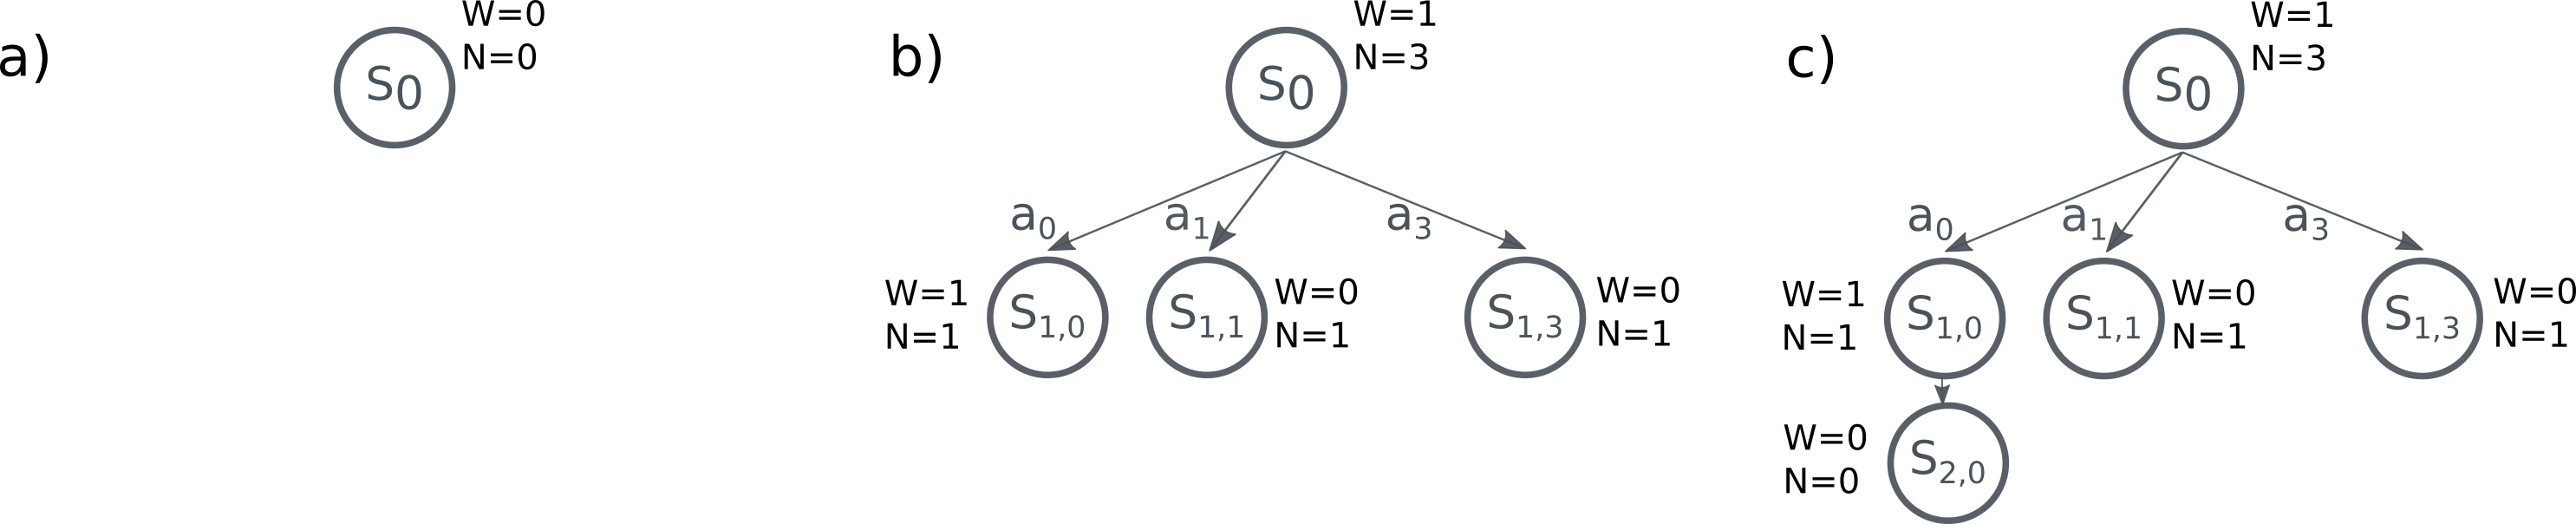
\includegraphics[width=\textwidth]{media/img/mctsTreeBuildPartOne}
	\caption{The first three phases of building a Monte Carlo Search Tree: (a) Set current state as root node (b) Initialise all legal moves of root state we can perform UCT (c) Selection of best action and expansion at first node not included in the tree.}\label{f:initTree}
\end{figure}
We then simulate a game for each legal action of that root node. This means we now have statistics for each action and its subsequent state. Figure \ref{f:initTree} part b shows the state $s_0$ as the root node, the legal actions as its branches, and the subsequent states of the actions as children nodes.

After initialising the tree we can enter the selection phase. This involves using an algorithm (refer Subsection \ref{s:tPolicy}) to pick the `best' child node as per the algorithm. This process is repeated with subsequent child nodes until we reach one without any statistics. Selecting these nodes presents a problem of exploiting actions with known good win rates and exploring alternative actions which might have better win rates. This problem is known as the multi-armed bandit problem and it has been studied extensively in literature and is discussed further in Section \ref{s:tPolicy}.

Reaching a node with no statistics means we enter the extpansion phase. The new node is added to the tree and is initialised with the statistics $N=0$ and $W=0$. Following on from the example shown in Figure \ref{f:initTree} part a, the expansion phase is illustrated in Figure \ref{f:initTree} part c. From there we enter the roll-out phase which means rapidly simulating the remaining moves of the game with a simple default policy (refer Subsection \ref{s:rollOut}) as depicted in Figure \ref{f:treeRollout}.
\begin{figure}
	\centering
	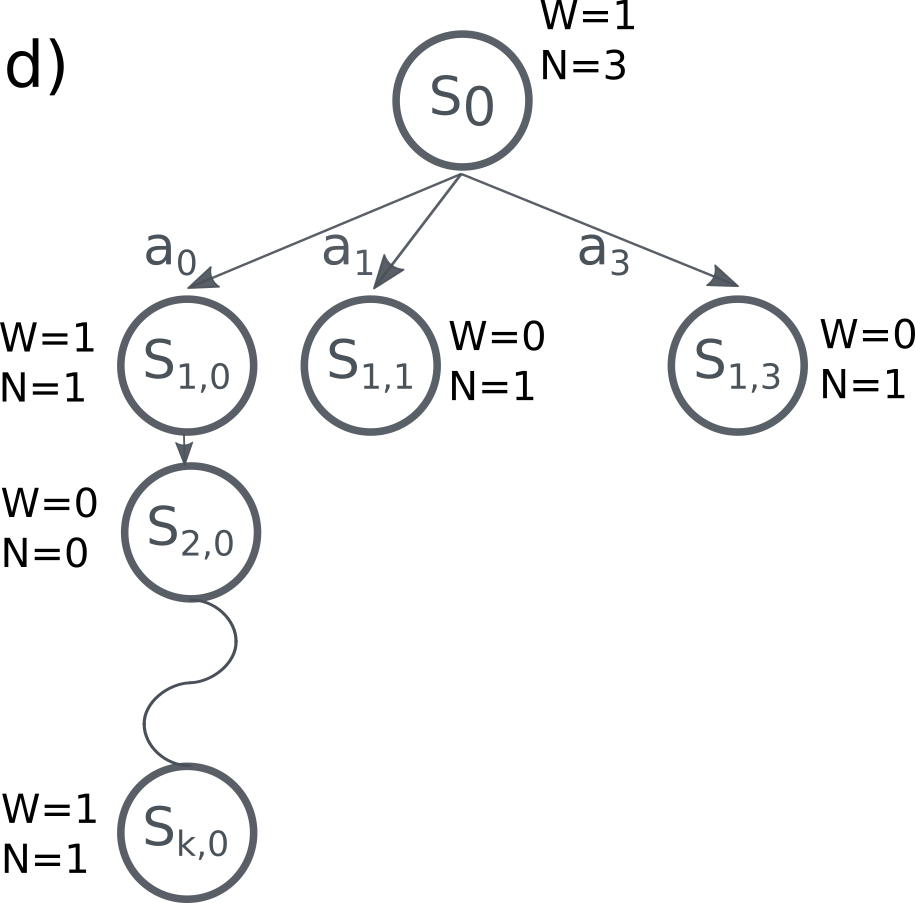
\includegraphics[width=.4\textwidth]{media/img/mctsTreeBuildPartTwo}
	\caption{The roll-out phase of a building a Monte Carlo Tree.}\label{f:treeRollout}
\end{figure} 
Once we reach the end of the game (terminal state), we can determine if we win or lose. As the name of the final phase suggest, this outcome is back-propagated up the sequence of moves carried out in the tree. For example, if the outcome was a win each node in this sequence would have its win and play count increased by one. This process is illustrated in Figure \ref{f:treeBackprop}, note that we do not have any expanded nodes in the roll-out phase so no statistics are recorded in that section.

\begin{figure}
	\centering
	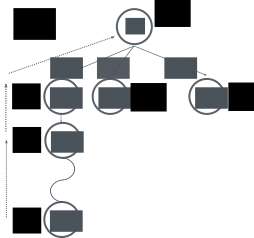
\includegraphics[width=.4\textwidth]{media/img/mctsTreeBuildPartThree}
	\caption{The back-propagation phase of a building a Monte Carlo Tree.}\label{f:treeBackprop}
\end{figure}

\subsection{Tree Policy}\label{s:tPolicy}
The multi-armed problem is when a gambler tries to maximise his cumulative reward from several slot machine (one-armed bandits). The gambler plays a slot machine to get a reward from some unknown probability distribution, the more he gambler plays, the more accurate he can estimate the distribution and therefore the expected (read average) reward. The gambler must decide which machine to play, how many times to play it, and when to switch to another. He must balance this in order to maximise his cumulative reward over all the slot machines played. 

The multi-armed bandit problem is a way of modelling the selection process of child nodes in a Monte Carlo tree. Many solution exist but the most common and successful one is the Upper Confidence Bound for Trees (UCT) \cite{Browne2012}. This uses the formula:

\begin{equation}\label{e:UCT}
Z(s,a) = \frac{W(s,a)}{N(s,a)} + C\sqrt{\frac{\log(N(s))}{N(s,a)}}
\end{equation} 


Where $N(s,a)$ is the number of times action $a$ has been selection from state $s$, $W(s,a)$ the number of times this action has resulted in a win at the terminal state, $N(s)$ is the total number of simulations played from state $s$, and $C$ is a tuning constant.

UCT is used to calculate the value of the child nodes and the one with the highest value is selected. This is repeated to follow a sequence through the current tree until we come to a node which has not been explored before. UCT comprises three main components; the exploitation factor $\frac{W(s,a)}{N(s,a)}$ representing the win rate, the exploration factor $\sqrt{\frac{\log(N(s))}{N(s,a)}}$ representing how many times a node has been selected, and the exploration constant $C$ which is tuned to the desired level of exploration. The exploitation factor is high for successful nodes and the exploration factor is high if they have been explored very few times. This means the UCT tree policy favours actions that result in wins but will still select actions if they have not been explored very many times.

There are many other bandit-based algorithms to potentially improve upon the tree policy and alternaitve upper confidence bound algorithms include UCB1-Tuned \cite{Auer2002}, Bayesian UCT \cite{Grunwald2010}, and EXP3 \cite{Auer1995} \cite{Audibert2009}. However, the policy is not the focus of this report is therefore not covered extensively. The papers for the alternative algorithms mentioned above are included in the references for the reader to view at their leisure.

\subsection{Roll-out}\label{s:rollOut}
The roll-out phase is designed for rapid play-out to reduce the overall computational expense of Monte Carlo Tree Search. This is achieved by having a default policy which can be as simple as always selecting the move location at position (0,0) in subsequent states until a terminal state is reached. A more common approach is sampling over a uniform random distribution of legal moves but they can also be tailored to suit the problem domain to dramatically improve performance \cite{Browne2012}.

\subsection{Other Enhancements}
There are further modification that can be done to Monte Carlo Tree Search to enhance it. One popular algorithm is rapid action value estimate (RAVE) and was introduced by MoGo, a 9 $\times$ 9 Go program \cite{Gelly2007}. RAVE solves the problems of initialising the tree (refer Section \ref{s:mcts}) by treating moves selected in subsequent states as if they selected from the root state (if they also exist from the root state).
This means that any moves from the root state that match those in the simulation can be given the same statistics. RAVE also introduces a decay factor so that this initialisation feature disappears as more simulations are carried out.

\section{Neural Networks and Deep Learning}\label{s:NN}
In this section we cover the background literature on neural network layers, convolutional networks, and deep learning.

\subsection{Neural Networks}
A neural network is a style of programming where programs learn from observing data. It can be thought of as a function which must first be taught how to do something so that it can give accurate answers. They are commonly used in state-of-the-art programs for image recognition, speech recognition, and natural language procession. In other words, they are excellent at classification and identifying patterns in complex data.

Neural networks are made up of an input, output, and one hidden layer as shown in Figure \ref{f:NN} and deep neural networks have more than one hidden layer. A neuron fires when the value of the output function goes above some threshold. This function is composed of weights, input values, and a bias and is given in Equation \ref{f:outputFunc}.

\begin{equation}\label{f:outputFunc}
o = w_ix_i - b_i
\end{equation}

Where $w_i$ is the weight, $x_i$ is the input, and $b_i$ is the bias. The output fires when it is above $0$ and the bias is the threshold value. Typically $w_i$ is tweaked in the training stage so the input data has an appropriate influence.


\begin{figure}
	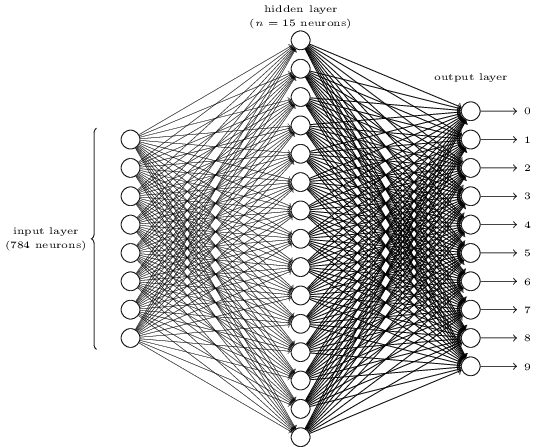
\includegraphics[width=\textwidth]{media/img/nnArch2}
	\caption{A neural network with 784 input values (only 8 shown), one hidden layer, and 10 output values for classifying numbers 0 to 9. \cite{Neilsen2015}}\label{f:NN}
\end{figure}


\subsection{Training Neural Networks}\label{s:nnTrainLit}
Training a neural network (NN) can take days or even weeks and different methods of doing this are common areas of current research. Training a network involves supervised learning which means that it will try to classify something and we tell how close it is to being correct. If it is not correct, the program is reversed and the weights connecting the neurons are changed by a small amount to make it more accurate. This is repeated millions of times until the NN is able to produce accurate results.

\subsection{Convolution Layer}
In this subsection we describe the convolution operation, how it is used in the convolutional layer and what advantages they have.

A convolution is essentially a weighted average. It can be used to detect vertical or horizontal edges in an image depending on the weights in the convolution. For example, imagine we have a very small $3 \times 3$ image as shown in Equation \ref{e:smallImage}, where each number is a pixel and the value represents a colour. Also shown is a filter, typically much smaller than the image but here is it as a $2 \times 2$ matrix.

We then compute the first convolution by placing the filter over the four top left numbers in the image which results in the operation shown in Equation \ref{e:convOp} and a single value of three. This is repeated three more times by sliding the filter across the image (the top-right four values, then bottom-left, then bottom-right) to get four values in total as shown in Equation \ref{e:convOp2}.

\begin{equation}\label{e:smallImage}
image = 
\left[ \begin{array}{ccc}
0 & 1 & 3 \\
2 & 1 & 4 \\
1 & 5 & 6 \\
\end{array}\right]
filter = 
\left[\begin{array}{cc}
1 & 2 \\
3 & 4 \\
\end{array}\right]
\end{equation}

\begin{equation}\label{e:convOp}
\left[\begin{array}{ccc}
0 \times 1 & 1 \times 2 & 3 \\
2 \times3 & 1 \times 4 & 4 \\
1 & 5 & 6 \\
\end{array}\right]
\Rightarrow
cell(0,0) = (1+2+6+4)/4 = 3
\end{equation}

\begin{equation}\label{e:convOp2}
Convolved Image=
\left[\begin{array}{cc}
3 & 5.5 \\
6.75 & 12 \\
\end{array}\right]
\end{equation}

The filter can have certain weights to detect edges, dark regions, and other attributes. If we now imagine a convolutional neural network we get something like the example illustrated in Figure \ref{f:CNNInput}. We repeat the previously described process on the input layer to produce the first hidden layer. The weights, depicted as lines in the illustration, are learnt by the neural network and shared for all neurons in the first hidden layer. One shared filter is called a feature map and allows you detect certain aspects of an image such as all the vertical edges. For each different aspect of an image you need another feature map and therefore convolutional neural networks are generally made up of several feature mappings. Figure \ref{f:CNN3Feature} shows three feature maps from the input layer to produce three different layers (channels) in the first hidden layer (3 channels of 24 by 24 neurons). Each layer would be detecting a different aspect of the image such as vertical, horizontal, and circular edges.

An advantage of a convolutional layer is that it takes into account the spatial structure of an image. This means it knows the top-left cell is next to the second top-left cell whereas in normal neural networks these two cells would be considered the same distance from each other as the top-left and bottom-right i.e. regular layers have no distance metric.

Another advantage is the sharing of weights for each filter map. This greatly reduces the number of parameters to learn therefore significantly reducing the time to train a network. Before incorporating convolutional layers it was considered to hard to train image classifiers as they contain too much data. Now, simple convolutional neural networks can be trained in minutes.

\begin{figure}
	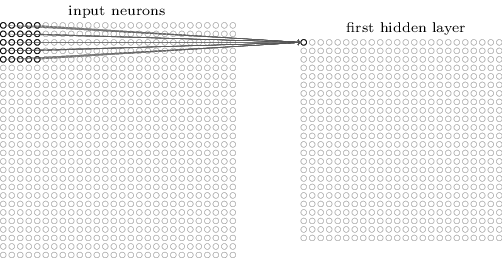
\includegraphics[width=\textwidth]{media/img/cnnInputAndHidden}
	\caption{Input and First Hidden Layer of a convolutional neural network \cite{Neilsen2015}}\label{f:CNNInput}
\end{figure}

\begin{figure}
	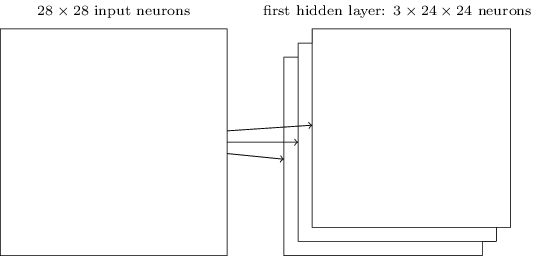
\includegraphics[width=\textwidth]{media/img/cnn3FeatureMaps}
	\caption{Three feature maps from the input layer \cite{Neilsen2015}}\label{f:CNN3Feature}
\end{figure}


\subsection{Max Pooling Layer}
Max pooling is typical pooling layer that occurs immediately after convolution layers. This layer is similar to a convolutional layer except the filter selects the maximum value rather than computing the weighted average. For example, if we have the same image as shown in Equation \ref{e:smallImage} and apply a two by two max-pooling filter to the four top left numbers we get a value of two as it is the maximum. This is repeated three more times to get the hidden layer as shown in Equation \ref{e:maxPool}.

\begin{equation}\label{e:maxPool}
maxPooledImage=
\left[\begin{array}{cc}
2 & 4 \\
5 & 6 \\
\end{array}\right]
\end{equation}

The advantage of this to reduce the number of parameters by even more without any significant loss in data quality.
\subsection{Drop-out Layer}
A drop-out layer is simply a training method to prevent over fitting. Over fitting is a term used to describe when a neural network predicts accurately on the training data but does not generalise well to unseen data. Drop-out prevents this by randomly selecting and temporarily deleting different connections between neurons of different layers as shown in Figure \ref{f:nnDropout}.

\begin{figure}
	\centering
	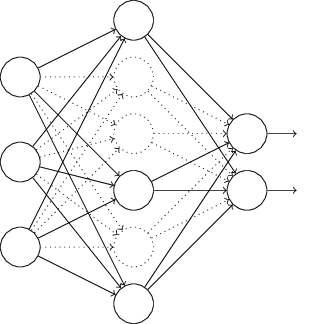
\includegraphics[width=.4\textwidth]{media/img/nnDropout}
	\caption{Drop-out in a neural network where the dotted lines indicate the temporarily deleted connections \cite{Neilsen2015}.}\label{f:nnDropout}
\end{figure}

For example, a 50\% drop-out essentially means each half of the NN will trained and able to classify the data independently. Then when it is used in practice, we no longer drop any connections and it is like having two NNs voting on the classification and we take the average as the result.



\chapter{Problem Domain}\label{ch:pb}
In this chapter we explain why Gem Island (refer Section \ref{s:gamed}) is classified as a POMDP (refer Section \ref{s:pomdb}) with stochastic elements.

Gem Island is a MDP (refer Section \ref{s:mdp}) as it requires a sequence of decision to reach a terminal state and each state transition involves a reward. The agent must find a sequence of actions to maximise the sum of these rewards. 

It is partially observable as each game is generated with five rows of ice with three medals hidden underneath. The medals are also randomly located as long as they do not overlap. An agent cannot see the medals until it removes the ice therefore, this hidden information indicates it is a POMDP.

Gem Island has stochastic elements due to the random gem generation. Each gem is generated by randomly assigning it a type with value between (and including) one to six. Both the gem generation and medal placement are sampled from a uniform distribution which means these elements are non-deterministic. This element makes it even more challenging for an agent to solve.

\chapter{Solution Design}\label{ch:solD}
In this chapter we discuss our agent design which will solve Gem Island. We apply current literature of Monte Carlo Tree Search (MCTS) and neural networks (NN) to reach a working solution. The problem domain can be found in Chapter \ref{ch:pb} and the MCTS and NN literature can be found in Sections \ref{s:mcts} and \ref{s:NN}. In our solution we introduce a number of MCTS designs each with different evaluation functions and they are:

\begin{itemize}
	\item No evaluation function
	\item Crude evaluation function
	\item Heuristic based evaluation function
	\item Evaluation network with outcome labels
	\item Evaluation network with utility labels
\end{itemize}

\section{Monte Carlo Tree Search}\label{s:mctsDesign}
In this section we outline the design of the modified selection and expansion process, the `opponent' modelling to account for the stochastic medal placements, and the roll-out and back-propagation phases.

Monte Carlo Tree Search works well in deterministic games because a tree can be built to store the win rate of state-action pairs and it is possible to reach the same subsequent states in following simulations. Building a tree is also useful for some non-deterministic games where the number of possible states from the previous state (branching factor) is relatively low. However, in Gem Island the branching factor is at minimum 216 (three gems) and can easily reach 10,000,000 (nine gems). In addition, the possible medal locations under the ice contribute to this branching factor. Furthermore, there is equal chance of reaching any one of those 10 million states. This means if we store a sequential state in the tree we have a very low likelihood of reaching the same state in a following simulation ($10^{-5}\%)$. If we make a move from this state and store it in the tree (level 2 in the tree) the chance of reaching it drops significantly to $10^{-10}\%$. We can see that after twenty levels it is extremely unlikely to reach the same state again. Because of this very low chance of reaching the same state we skip the expansion phase in our MCTS design. Rather we only store the legal actions from the root state and their corresponding win and play counts. This means we use the roll-out phase with the default policy (refer Section \ref{s:rollOut}) for the remaining moves. This design is referred to as Flat UCB in literature \cite{Coquelin2007} and is illustrated in Figure \ref{f:mctsImplementation}. A benefit of this is efficient memory storage as only one level of actions is stored and we ignore the encoded state (refer Section \ref{s:state}). Furthermore, this reduces the back-propagation process from iterating over all expanded nodes in the sequence to simply adding the win and play count directly to the first action.

\begin{figure}
	\centering
	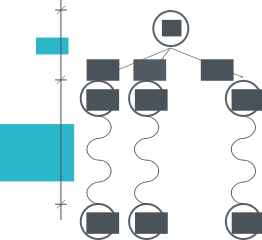
\includegraphics[width=.6\textwidth]{media/img/mctsImplementation}
	\caption{Monte Carlo Tree Search with a Flat UCB design.}\label{f:mctsImplementation}
\end{figure}

The algorithm used for the Flat UCB design is outlined in Figure \ref{l:FlatUCB} which is based upon Algorithm two in Browne et al's paper \cite{Browne2012}


\begin{figure}[h]
	\centering
	\begin{verbatim}
	function FlatUCB(s0)
	  create root node v0 with state s0
	  while within computational budget do
	    vl = TreePolicy(v0)
	    update = DefaultPolicy(s(vl))
	    Backup(vl, update)
	  return a(BestChiled(v0,0))
	
	function TreePolicy(v)
	  bestChild = argmax(v' children of v) W(v')/N(v') + c.SQRT(2lnN(v)/N(v'))
	  return bestChild
	  
	function DefaultPolicy(s)
	  moveLimit = n
	  count = 0
	  while s is non-terminal or count < moveLimit do
	    chose a legal action unformly at random, a
	    s = state reached from selecting action a from state s
	    count = count + 1
	  return reward for state s
	
	function Backup(v, update)
	  N(v) = N(v) + 1
	  W(v) = W(v) + update
	
	\end{verbatim}\label{l:FlatUCB}
	\caption{The Flat UCB algorithm used in the author's MCTS.}
\end{figure}




\section{No Evaluation Function}\label{s:noEval}
The first design is a full Monte Carlo Tree Search without an evaluation function. This means the roll-out phase is played until the a terminal state and the action selected from the root state has its win and play count updated according to the outcome. We did not expect this to perform well as it does not realise partially uncovering medals is helpful.

\section{Crude Evaluation Function}\label{s:crudeF}
This design incorporates a crude evaluation function which gives a state a rating in the range of zero to one, where one represents a certain win. This also means the roll-out phase can go to any depth, such as one look-ahead or fives moves, rather than until a terminal state. The function is considered crude as its only feature is to count the portion of medals remaining. The portions count is normalised by dividing it by the total portions remaining in the root state and this function is shown in Equation \ref{e:crude}. This feature was chosen as removing all the medals is the goal of the game and is therefore the most important feature. We expected this to perform well as it can now determine that partially uncovering medals leads to success.

\begin{equation}\label{e:crude}
crude(mp) = \frac{mp}{mp_{remaining}}
\end{equation}

Where $mp$ represents medal portions.

\section{Heuristic Based Evaluation Function}\label{s:hbF}
The heuristic based (HB) evaluation function is similar to the crude version except it includes additional features. We decided upon the features of medal portions uncovered, ice removed compared to the root state, and the number of different gems compared to the root state. These features are designed to encourage exploration under the ice, remove as many gems as possible, and to finish the game quickly. In doing so we hoped to increase the overall win rate of the AI.

Finding the correct weights of these features involved much trial and error. We began with coarse grained tuning of the weights which involved running a set of values for 20 to 50 simulations. Once we determined a rough range of values that resulted in a performance comparable to the crude function we switched to fine grained tuning. This involved tweaking the weights by small amounts and each set of values was run 100 to 300 times. The final HB function is shown in Equation \ref{e:HB}. Where $ir$ is the amount of ice removed and $gr$ is the number of gems changed from the root state.

\begin{equation}\label{e:HB}
HB(mp, ir, gr)  = \frac{10}{16}\times mp + \frac{5}{16}\times ir + \frac{1}{16}\times gr
\end{equation}

\section{Evaluation Network with Outcome Labels}\label{s:nnOL}
The Evaluation network with outcome labels is a simple neural network with a convolutional layer with 6 feature mappings and a 50\% drop-out layer. The architecture of this network is illustrated in Figure \ref{f:nnArch}.

\begin{figure}
	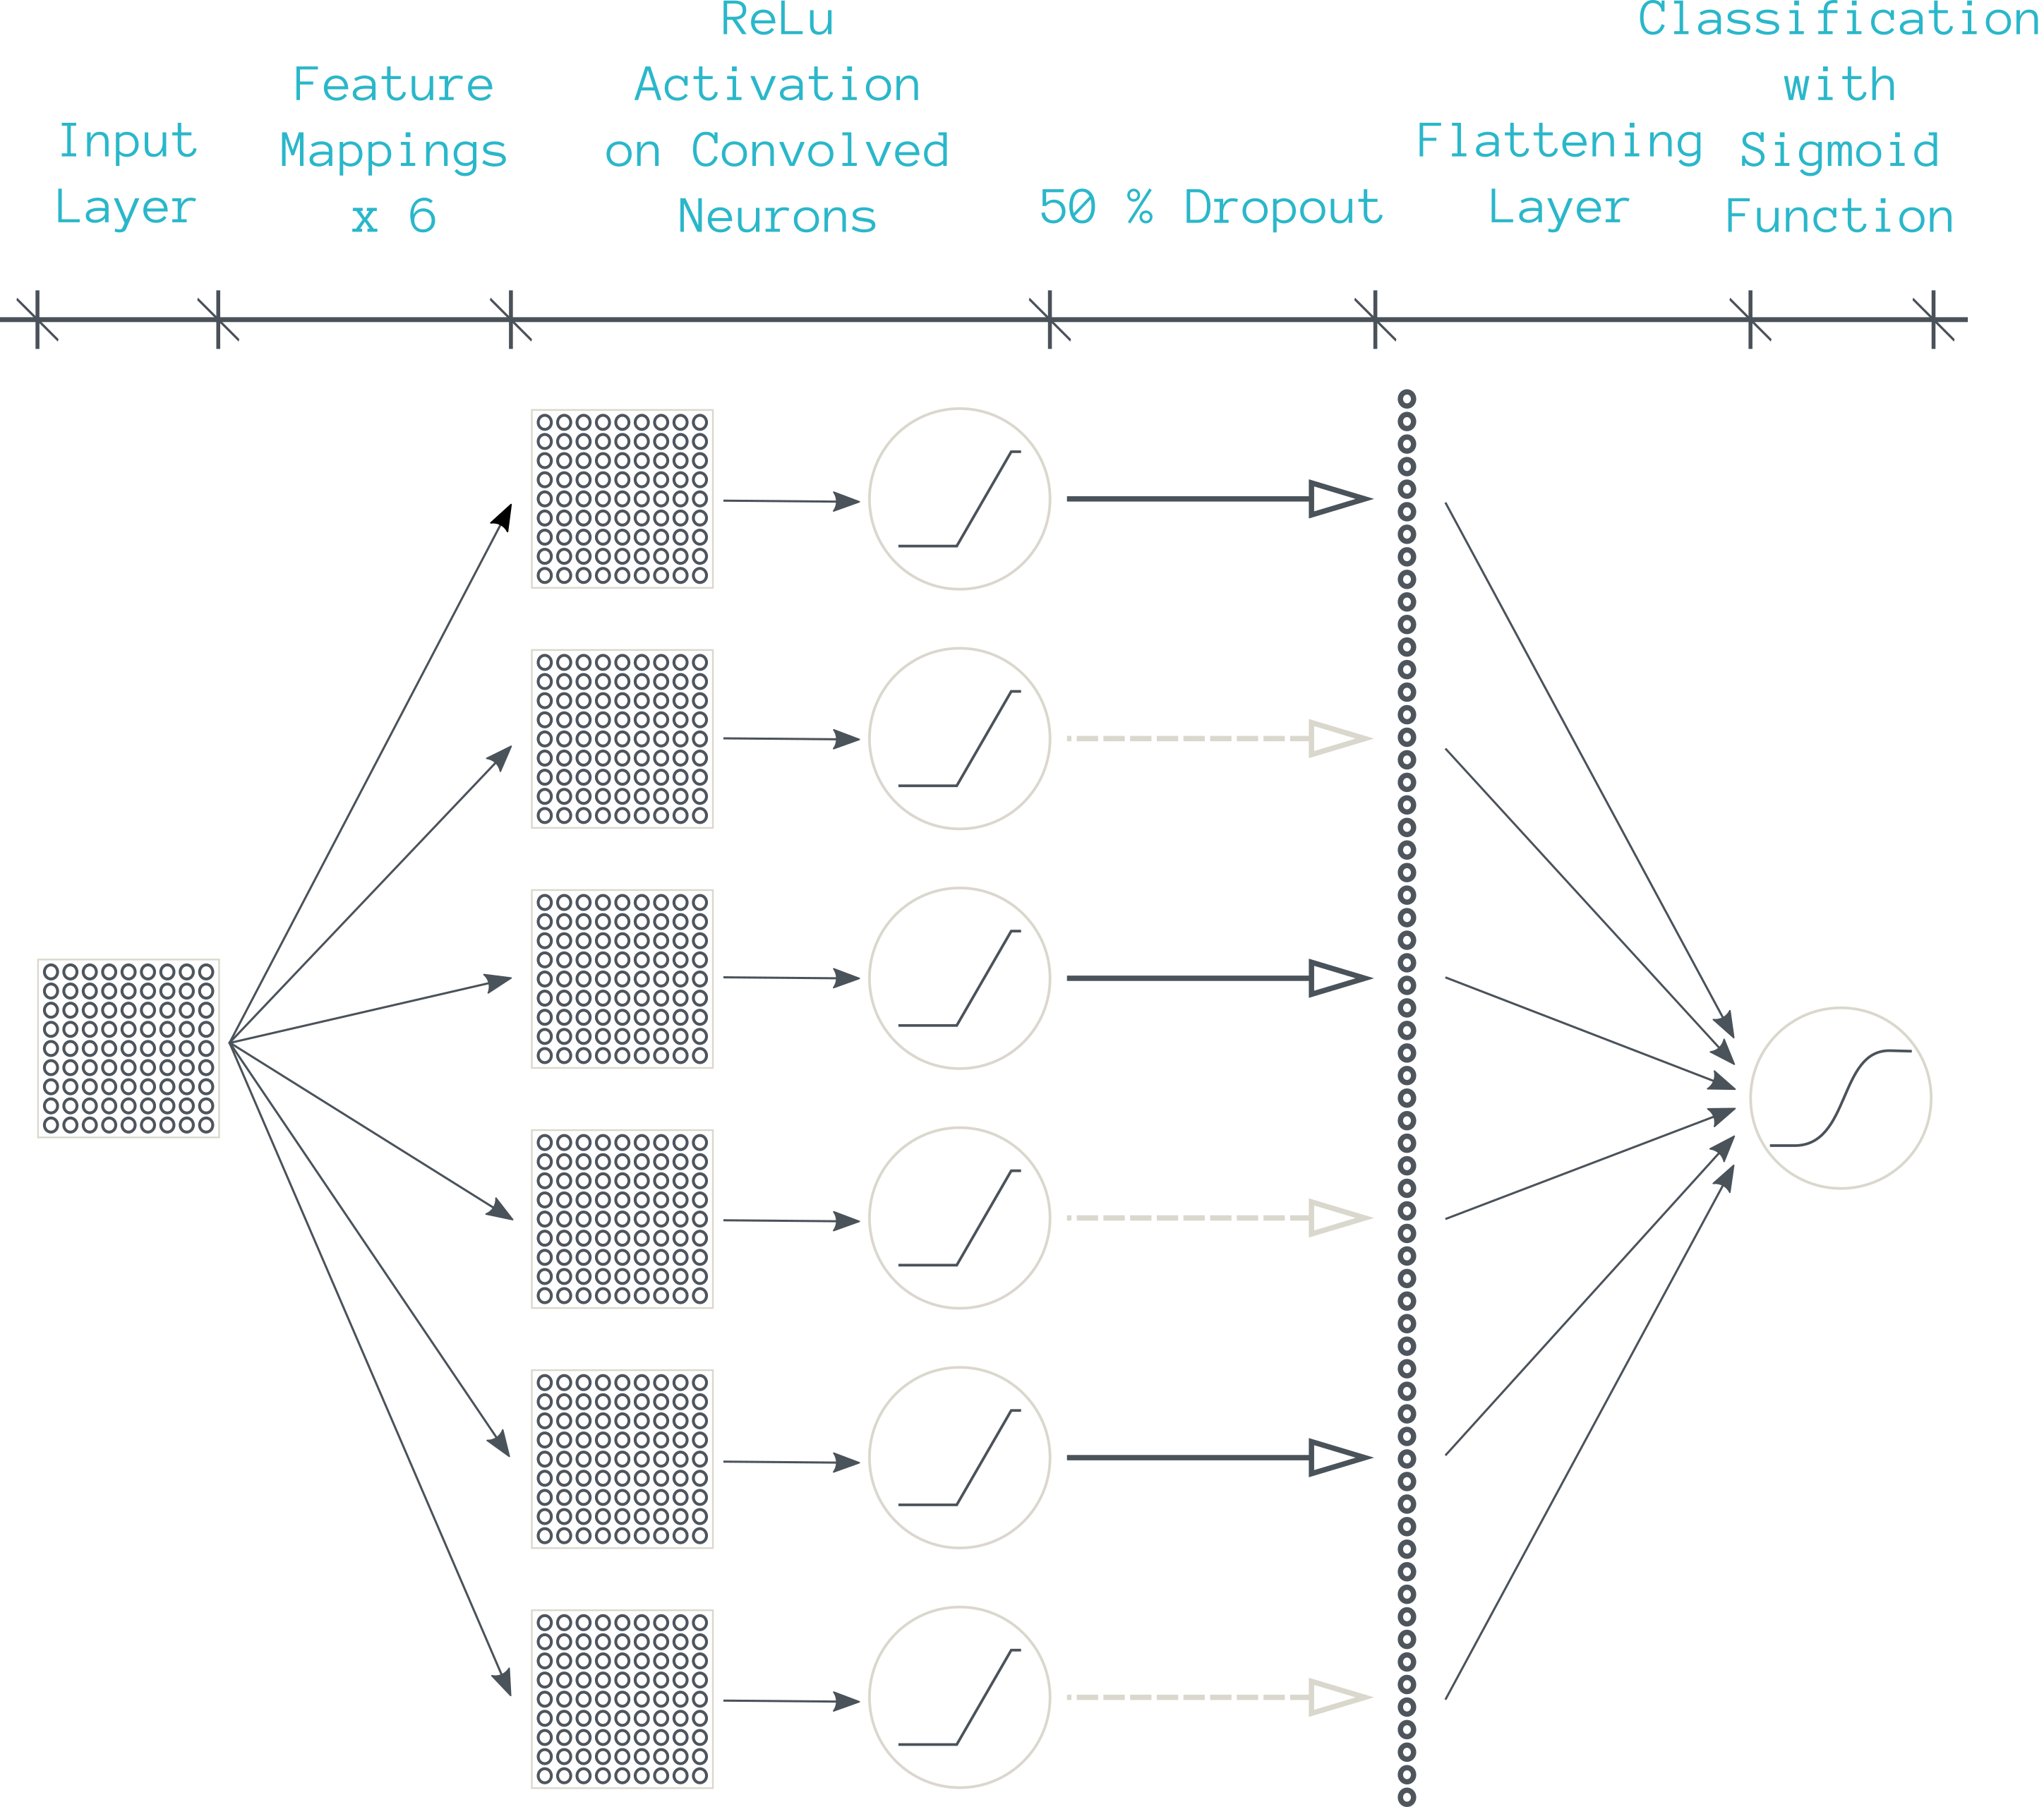
\includegraphics[width=\textwidth]{media/img/nnArch}
	\caption{The architecture of the evaluation network trained with outcome labels.}\label{f:nnArch}
\end{figure}
 The network was trained by randomly selecting one state (refer Section \ref{s:state}) per game from the six thousand games that were recorded from the website (refer Section \ref{s:website}). Only one state was selected from each game to avoid any correlation between subsequent states. The states were changed into fourteen one-hot encoded states to make training the network simpler. This means the six gem types are now split into by six different layers where the first layer is a $9 \times 9$ array composed of ones if a type one gem existed at that position and zero if not. An example of this is shown in Figure \ref{f:oneHot}. The next three layers represent the bonus types, one layer for ice, and four layers for medal portions. An interpretation of how this would look is illustrated in Figure \ref{f:nnTraining}.
 
\begin{figure}
	 \begin{equation}
 \left[\begin{array}{ccccccccc}
 1 & 1 & 0 & 0& 0& 0& 0& 0& 0\\ 
 1 & 1 & 0 & 0& 0& 0& 0& 0& 0\\ 
 0 & 0 & 0 & 1& 0& 1& 1& 0& 0\\ 
 0 & 1 & 0 & 0& 0& 0& 0& 0& 0\\ 
 1 & 1 & 0 & 0& 0& 0& 0& 0& 0\\ 
 1 & 0 & 0 & 0& 0&1& 0& 0& 0\\ 
 0 & 0 & 1 & 1& 0& 0& 0&1& 0\\ 
 0 & 0 & 0 & 0& 0& 1& 0& 0& 0\\ 
 0 & 0 & 0 & 0& 0& 0& 0& 1& 1\\ 
 \end{array}\right]
 \end{equation}
	\caption{An example of a $9 \times 9$ one-hot encoded array.}
	\label{f:oneHot}
\end{figure}
 
 \begin{figure}
 	\centering
 	
\includegraphics[width=0.5\textwidth]{media/img/nnTraining}
 	\caption{The one-hot encoded states for training the neural networks.}\label{f:nnTraining}
 \end{figure}
 
For each state we have the outcome of that game which is what was used as the training labels. This means if state $s_n$ belonged to a game which resulted in a win it would be assigned a label of one and zero if it was a loss. These corresponding labels were stored in a one-dimensional array as shown in Figure \ref{f:nnLabels}.

 \begin{figure}
	\centering
	
\includegraphics[width=0.13\textwidth]{media/img/nnLabels}
	\caption{The corresponding labels for the training data.}\label{f:nnLabels}
\end{figure}

There is also a risk of over-fitting (refer Section \ref{s:nnTrainLit}) to the gem types rather than the pattern of gems. To avoid this we permuted the states to get every every combination and to make it gem type agnostic. Consequently this increased our training data by a factor of 720.
We expected this network to perform reasonably well as it should learn what local gem patterns lead to a win. However, it did not and this is discussed in the results in Section \ref{s:resultsC}.

\section{Evaluation Network with Utility Labels}\label{s:nnUL}
This network used a similar design to make it comparable to the outcome label network, however, instead it used what we named utility labels. These labels were computed by running Monte Carlo Tree Search on each state and selecting the maximum action win rate. In other words it works out the likelihood of winning from an arbitrary state.
We expected this evaluation network to perform very well however due to time constraints it was not carried out but it remains a possibility for future work.

\chapter{Technical Requirements}\label{ch:techReq}
To build an agent to win match three we also needed an open source version of the game so we could get the game state and control it with AI. Therefore we designed and implemented our own version which is outlined in Section \ref{s:gamed}. 

To train the neural network we needed data. To gather this data we built a website that recorded users moves and logged it all in files on the server. The design of the website is outlined in Section \ref{s:website}.

\section{Game Design: Gem Island}\label{s:gamed}
In this section we outline the game design, design patterns used, the game logic, and sprite animation.


The board in Gem Island is a $9 \times 9$ grid of cells. Each cell can contain a gem, ice, or a medal portion. The ice is always generated in the bottom five rows with one layer (only one match to remove ice) as shown in Figure \ref{f:gemIsland}. Three medals are randomly placed under the ice at the beginning of the game and must not overlap each other. To win a game all the medals must be freed. To free a medal all the ice covering it must be removed and to remove ice a match must be made on top of it. A match is three or more gems of the same type in a succession. To make a match a user (or agent) must swap two adjacent gems. Only legal moves are allowed where a legal move means it must result in at least one match. Each medal always has four portions numbered zero to three from the top-left to the bottom-right (square). Figure \ref{f:gameUncoveredMedals} shows the state of a game with some portions uncovered. There are three possible bonuses and the way they are earned are as outlined in the rules below as well as their effects.

 \begin{figure}
	\centering
	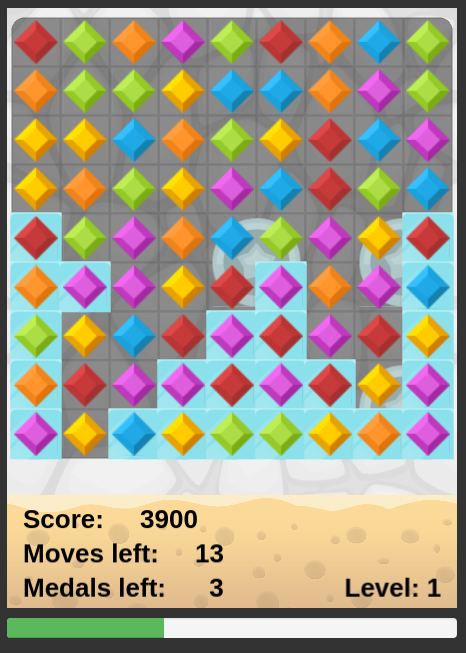
\includegraphics[width=0.4\textwidth]{media/img/screen3Medals}
	\caption{A game of Gem Island with some silver medals partially uncovered.}\label{f:gameUncoveredMedals}
\end{figure}

\subsection{Game Rules}
\textbf{Goal}: To remove all the medals.\\
\noindent\textbf{Gem Types}
\begin{itemize}
	\item 6 gem types.
	\item 3 bonus types (star, cross, diamond).
\end{itemize}
\textbf{Earning Bonuses}
\begin{itemize}
	\item If a bonus gem removes another bonus gem, it also performs its bonus action. This is done recursively.
	\item 3 or more gems in a succession of the same type is a match.
	\item 5 gems in a succession earns you a star bonus.
	\item An intersection of a vertical and horizontal match earns you a diamond bonus.
	\item If a match generates multiple bonuses only one is generated following the hierarchy: star, cross, diamond.
\end{itemize}
\textbf{Bonus Actions}
\begin{itemize}
	\item Star bonus removes all gems of the star gem's type.
	\item The cross bonus removes all gems in the row/column. If the match is horizontal, the row is removed. Vertical removes the column.
	\item The diamond bonus removes the 9 surrounding gems of the diamond gem.
\end{itemize}

\subsection{Game Code Design}

The overall design pattern used was Model View Controller (MVC), where the model contained the game logic and sent the state and movement information to the view. This information was wrapped in a container class named \verb|UpdateBag|. The view was designed to be naive, in the sense that it only arranged the graphics on the screens as per the information sent in the \verb|UpdateBag|. The view also handled loading in the sprites (gem, ice, and medal graphics) and the animations of exploding and moving gems.

Several different controllers were used but they all controlled the game by sending \verb|SwapGemsRequest| objects to the model. The \verb|SwapGemsRequest| class is designed to contain two coordinates to indicate the gems to be swapped. The \verb|MouseController| class listens for mouse events, such as the user clicking and dragging, and sends them via a \verb|SwapGemsRequest|. The \verb|NaiveAIController| reads in the encoded states, selects a legal move at random, and sends a swap request.
Finally, the \verb|MCTSController| class is designed to read in the encoded states, run one of the various MCTS implementations, and send a swap request.

The communication between the model, view, and controller classes was handled by an event manager class: \verb|EventManager|. The event manager class was passed into each of the model, view, and controllers so they could `register' themselves. Every registered class could now received events and requests via their own notify method, which \verb|EventManger| called by looping over the registered objects. Additionally, they could all send events and requests by calling the \verb|post| method on the passed in \verb|EventManager| object.

The model class was split into a parent and child class. The parent class contained the logic and could be used by the AI to simulate games quickly without any graphics. The child class contained additional methods for communicating with the view, such as to compute movement coordinates for the animations.

The model and view are designed to be dynamically sized allowing the gem grid to be any $m \times n$ size. Furthermore, any number of ice rows, layers of ice, and medals could be added. Figure \ref{f:gemRect} shows a $7 \times 16$ grid to illustrate the dynamic properties. A benefit of this dynamic design is the game can be changed to any difficulty therefore it can be made more challenging for the AI or user.


\begin{figure}
	\centering
	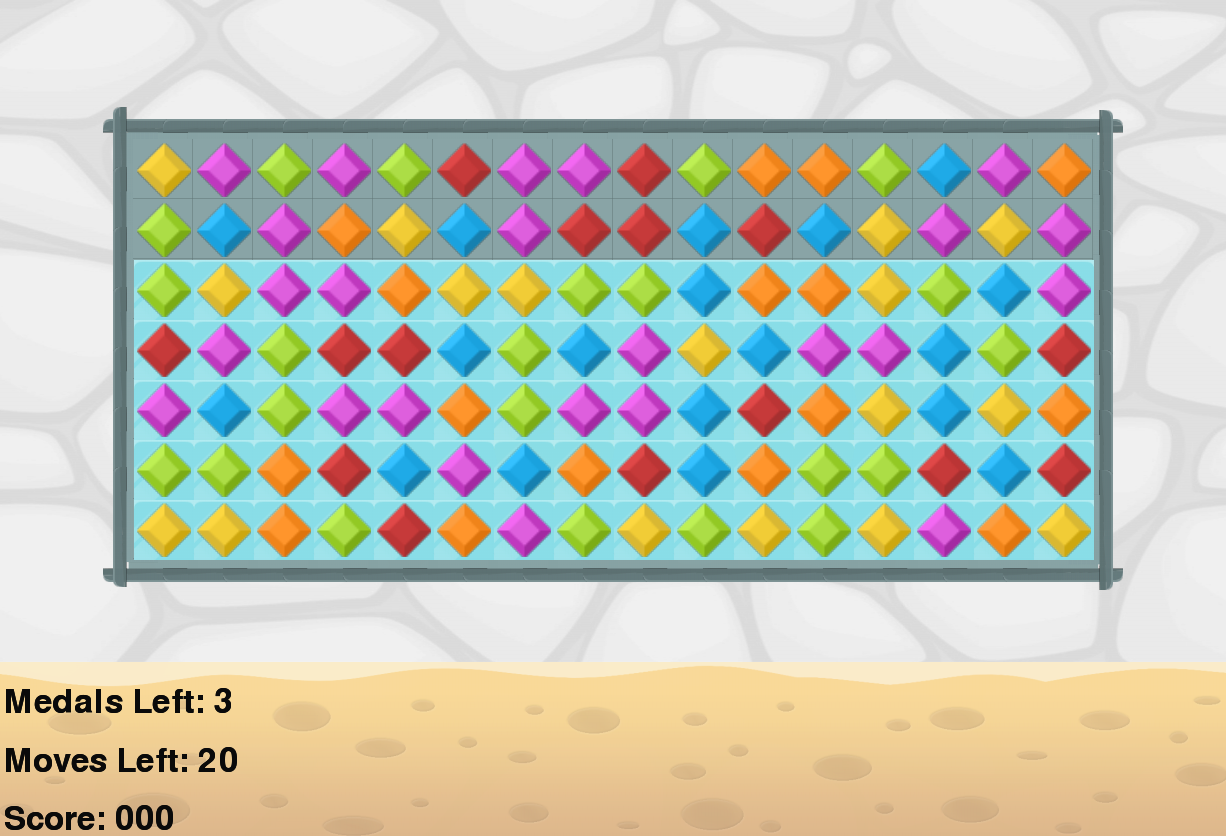
\includegraphics[width=\textwidth]{media/img/gemIslandRect}
	\caption{A Game of Gem Island with 7 rows and 16 columns.}\label{f:gemRect}
\end{figure}

\section{State Representation}\label{s:state}
The AI program must be able to read the current state of the game. This means the arrangement of the gems, ice, and medals must all be encoded so the program can determine what is shown on screen. For this we chose a simple string representation where a sequence of four numbers represented one cell in the $9 \times 9$ grid. The four numbers represented the gem type (colour), the bonus type, if ice is present, and a medal portion if it exists. This sequence of four numbers was repeated 81 times to represent each cell in the grid. The AI program could then decode this state string and simulate games via the Monte Carlo Search Tree.

\section{Testing and Validation}
In this section the unit tests used to test the game logic are listed. Only the title and description of each are included, for the full code refer to the URL below.

Test file:\\
 \verb|https://github.com/tombrereton/threematch/blob/master/tests/game_test.py|


\subsection{Bonus Creation Tests}


\begin{verbatim}
def test_create_diamond_bonus():
  """
  Test creation of diamond bonus.

  Vertical is a three in a column.
  Horizontal is a three in a row.

  The swap makes the horizontal and vertical
  intersect. The intersection is a
  diamond bonus (type 3).

  All matches should be removed including the gems
  from the bonus action (points (1,1) and (1,3))
  """
\end{verbatim}


\begin{verbatim}
def test_create_and_use_cross_bonus():
  """
  Tests the use and creation of a cross bonus.

  5 gems in a row. 3 gems of type 0.
  Then 1 gem of type 0 and cross bonus (removes entire row).
  Then gem of type 1.

  Should remove all gems in row and create a bonus at 1st swap location.

  Swap location is the zeroth element, and the bonus created should be
  type 1.
  """
\end{verbatim}:

\begin{verbatim}
def test_create_cross_over_diamond_bonus():
  """
  Tests creation of cross bonus over diamond bonus.

  Vertical and horizontal matches intersect but one is 4 long.
  This means a cross should be created rather than a diamond.
  """
\end{verbatim}



\begin{verbatim}
def test_create_cross_from_star_bonus():
  """
  Testing that a cross bonus is still
  created when using a bonus type 2.
  8 gems in a row.

  All gems of type 0 should be removed and a
  bonus of type 1 should be created at location (0,0).

  Bonus type 1 occurs from 4 in a row.
  Bonus type 2 destroys all gems of that type.
  """
\end{verbatim}

\subsection{Bonus Activation Tests}
\begin{verbatim}
def test_use_star_bonus():
  """
  Testing that a star bonus (type 2)
  removes all gems of the same type.

  5 gems in a row.
  2 gems of type 0. Then gem of type 0 and bonus type 2 (star).
  Then gem of type 1. Then gem of type 0.

  4 Gems should be removed (all of type 0).
  """
\end{verbatim}



\begin{verbatim}
def test_cascade_bonus_activations():
  """
  Testing cascade of bonus activation.

  Star bonus should remove all type 0 gems,
  one of which is a cross bonus, which should
  remove the remaining type 1 gem.

  5 gems in a row.

  1st gem is a diamond of type 0. 2nd is a gem of
  type 1. 3rd is a star of type 0. The last 2
  are normal gems of type 0.

  The star should remove all gems of type 0, which
  should the activate the 1st gem bonus, removing the
  type 1 gem.

  In short, this should remove all gems.
  """
\end{verbatim}



\begin{verbatim}
def test_using_cross_bonus_vertically():
  """
  Testing cross bonus removes column when
  in vertical match.

  5 gems in a column. 2 gems of type 0,
  then a gem of type 1, then a cross gem of
  type 0, then a gem of type 1.

  All 5 gems should be removed.
  """
\end{verbatim}



\begin{verbatim}
def test_using_cross_bonus_horizontally():
  """
  Testing cross bonus removes row when
  in horizontal match.

  5 gems in a row. 2 gems of type 0,
  then a gem of type 1, then a cross gem of
  type 0, then a gem of type 1.

  All 5 gems should be removed.
  """
\end{verbatim}


\subsection{Ice Removal Tests}
\begin{verbatim}
def test_ice_removed():
  """
  Testing that all ice is removed
  when gems are matched on top.

  All gems should match and remove
  the ice underneath.

  Grid is 2 by 3.
  """
\end{verbatim}

\begin{verbatim}
def test_remove_ice_when_creating_bonus():
  """
  Testing that ice is removed when a bonus is
  also created.

  Row of 4 gems of type 0.

  Should remove all gems except for the first,
  where a bonus of type 1 is created.

  The ice should all be removed underneath
  """
\end{verbatim}

\subsection{Game State Tests}

\begin{verbatim}
def test_get_game_state():
  """
  The get game state function should
  return all three states as a string in vector form.

  Medals are obscured so they should be all -1 values.
  """
\end{verbatim}

\begin{verbatim}
def test_get_game_state_2():
  """
  The get game state function should
  return all three states as a string in vector form.
  """
\end{verbatim}

\begin{verbatim}
def test_get_game_state_3():
  """
  The get game state function should
  return all three states as a string in vector form.
  """
\end{verbatim}

\section{Source Code Collaboration}
This project was undertaken in collaboration with another Student, Elliott Davies. This section includes Table \ref{t:sourceCode}, which outlines how the source code was divided between the two of us.

\begin{table}[]
	\centering
	\caption{The work allocation for this project.}
	\label{t:sourceCode}
	\begin{tabular}{lll}
		\hline
		Section                  & Python Main Author & JavaScript Main Author \\ \hline
		Model                    & Thomas Brereton    & Elliott Davies         \\
		View                     & Elliott Davies     & Thomas Brereton        \\
		Controllers              & Thomas Brereton    & Thomas Brereton        \\
		Event Manager and Events & Thomas Brereton    & -                      \\
		Monte Carlo Tree Search  & Elliot Davies      & -                      \\
		Evaluation Functions     & Thomas Brereton    & -                      \\
		Policy                   & Elliott Davies     & -                      \\
		Value Network            & Thomas Brereton    & -                      \\
		Policy Network           & Elliott Davies     & -                     
	\end{tabular}
\end{table}



\section{Website Design}\label{s:website}

The website was designed and constructed for users to play Gem Island on either there computer or phone. It was required so we could record the games and gather training data for the neural networks (refer Section \ref{s:nnTrainLit}). We recorded the files by sending an encoded state and the actions back to the server, which wrote it in a log file.

The overall design was a distributed design with the game running on the client (user's browser) and only the database and file manipulations would be handled on the server. The game was therefore re-written in JavaScript so it could run in the browser. This design was made as it was deemed easier than setting up a full python based server application and also the current Python implementation sends \verb|UpdateBags| for each movement of one cell, which would cause delays and stuttering. This would degrade from the game quality and discourage users to play.

To encourage people to play we created three levels with the variations as outlined in Table \ref{t:gameLevels}. Another incentive we designed was a high score table for the top fifty users of each level. This turned out to be very successful in encouraging users to play.

\begin{table}[]
	\centering
	\caption{Gem Island Levels}
	\label{t:gameLevels}
	\begin{tabular}{cccc}
		\hline
		Level & Ice Rows & Total Medals & Total Moves \\ \hline
		1     & 5        & 3            & 20          \\
		2     & 7        & 4            & 25          \\
		3     & 9        & 5            & 30         
	\end{tabular}
\end{table}



Writing the state-action pairs to file and saving the users high scores required server side programs. These were written in PHP and they handled the database queries and the writing of the state-action pairs to file. PHP was used as it works well with web programming languages such as JavaScript and made building the website simple.

Sending client side data to the server always involves risk and all data must be considered malicious. Therefore, security measures were designed. This included sanitising SQL queries before inserting into the database. This prevented cross site scripting (XSS) and SQL injection. Furthermore, we ran regex (regular expression) pattern matching on the state-action pairs before writing to disk. This ensured we only received data in the format we desired and prevented users from potentially writing malicious scripts to corrupt the server. Additionally, we minimised the impact of denial of service (DoS) attacks by only allowing requests to be sent to the server every two seconds. This was deemed appropriate as a user is unlikely to make a move in less than two seconds.

\chapter{Artificial Intelligence Performance Analysis}\label{ch:aiAnalysis}
In this chapter we outline the methodology used to perform the analysis. We then comment on the results and compare the performance of the various evaluation functions.

\section{Analysis Methodology}\label{s:analMeth}
Each experiment began with a game generated as per Section \ref{s:gamed} and a variation of the Monte Carlo Tree Search (MCTS) program was executed until it won or lost a game. Each variation was repeated a certain number of times to gather an adequate sample size as shown in Table \ref{t:MCTSConfig}. Note that some of the variations failed consistently therefore they were repeated fewer times. The MCTS parameters are also outlined in Table \ref{t:MCTSConfig} where Move Depth is how many moves are made per simulation, Game Limit is the number of simulations before selecting a move, C is the exploration constant. 

\begin{table}[]
	\centering
	\caption{The MCTS parameters and the number of times each variation was completed}
	\label{t:MCTSConfig}
	\begin{tabular}{lrrrr}
		\hline
		Evaluation Function    & Times Completed & Move Depth & Game Limit & C   \\ \hline
		None                   & 100             & 20         & 100        & 1.4 \\
		Crude                  & 300             & 5          & 100        & 1.4 \\
		Heuristic Based        & 300             & 5          & 100        & 1.4 \\
		NN with Outcome Labels & 100             & 5          & 100        & 1.4
	\end{tabular}
	\end{table}

The configuration for Gem Island is shown in Table \ref{t:analysisConfig}. As per Section \ref{s:gamed}, the gem types and medal locations are generated randomly at the beginning of each game. 

\begin{table}[]
	\centering
	\caption{The Gem Island Configuration for the Analysis}
	\label{t:analysisConfig}
	\begin{tabular}{lc}
		\hline
		Parameter    & Value \\ \hline
		Rows         & 9     \\
		Columns      & 9     \\
		Ice Rows      & 5     \\
		Ice Layers   & 1     \\
		Total Moves  & 20    \\
		Total Medals & 3    
	\end{tabular}
\end{table}


\section{Results and Comparison}\label{s:resultsC}

\begin{table}[]
	\centering
	\caption{MCTS variations and their win rates}
	\label{t:MCTSWinRates}
	\begin{tabular}{lrrr}
		\hline
		Evaluation Function    & Win Rate & Mean Moves Made & Mean Score \\ \hline
		Random                 & 0 \%     & 20              & 33,809     \\
		None                   & 33 \%    & 17.9            & 65,441     \\
		Crude                  & 85 \%    & 12.8            & 142,855    \\
		Heuristic Based        & 87 \%    & 12.5            & 167,783    \\
		NN with Outcome Labels & 21 \%    & 18.8            & 51,415    
	\end{tabular}
\end{table}

The results from the experiments performed as per Section \ref{s:analMeth} are shown in Table \ref{t:MCTSWinRates}. For a baseline, one hundred games were played by randomly selecting a legal move and the results have been included as the first row in the table under the evaluation function name of Random. The win rate of 0\% for selecting random moves also provides evidence that it is a non-trivial game and requires intelligence to solve it.

From Table \ref{t:MCTSWinRates} we can see the Heuristic Based (HB) evaluation function (refer Section \ref{s:hbF}) performed best with a win rate of 87\% and a mean moves made (MMM) of 12.5. This is only slightly better than the Crude function (refer Section \ref{s:crudeF}) which is unsurprising as medal portions uncovered is the most important feature to win the game. The HB function also included two additional features, ice and gems removed. This slight increased win rate and slight decreased MMM importantly indicates that these features do not subtract from the success and given more time to tune the parameters it may have performed better. As per the results, we can conclude that removing ice and gems assists in success of the function. This is likely due to the agent acquiring more information when removing ice and the removal of more gems gives a greater chance of random combinations which lead to medal removals. This logic follows along the lines of the quote by Kaelbing et al in Section \ref{s:pomdb} on POMDPs, where optimum moves must balance between maximising reward and acquiring more information.

No evaluation function and the NN with outcome labels (NNOL) both perform badly but are still better than randomly selected moves. It shows that an MCTS with a full roll-out and no evaluation function can only complete the game with a win rate of 33\% and MMM of 17.9. This is likely due to the lack of domain knowledge and indicates some of this knowledge is required to achieve a high win rate. Interestingly, the NNOL performs worse than no function with a win rate of 21 \%. This is likely due to the method in which it was trained. It was trained so that a states $s_0$ (start) and $s_{20}$ (terminal) of the same game which results in a loss will have labels of 0. However, $s_0$ will have zero medal portions uncovered and $s_{20}$ will likely have eight medal portions uncovered. $s_{20}$ clearly has a higher value than the initial state due to the amount of portions uncovered. This means the neural network is not learning to uncover medals as the labels give no indication that uncovering them is important.

If we compare the performance of the HB function with humans we see that it is approximately equal to the human players, if not better on average. The win rate of the top players that have played more than fifty games are shown in Table \ref{t:humanWinRates}. `Astrophysicist' achieved a much higher win rate compared to others with a rate of 89\%, which is only 2\% better than the MCTS with HB function. Considering all top players, the program achieved significantly better than average human playing ability and comparable to the human elite.

\begin{table}[]
	\centering
	\caption{The top human players for level 1 of the website}
	\label{t:humanWinRates}
	\begin{tabular}{lrr}
		\hline
		Nick name      & Win Rate & Game Played \\ \hline
		Astrophysicist & 89 \%    & 118         \\
		InputNameHere  & 69 \%    & 65          \\
		Elliott        & 68 \%    & 82          \\
		Gillyb         & 37 \%    & 931         \\
		default        & 35 \%    & 147        
	\end{tabular}
\end{table}


\chapter{Evaluation of Project}
In this chapter we discuss the limitation of the author and evaluate the difficulty and usefulness of the project.
To evaluate the project we must first mention the authors limitations and background. The author did not undertake the modules for Introduction to Artificial Intelligence and Neural Networks which covered both Monte Carlo Tree Search (MCTS) and convolutional neural networks (CNN). This meant the author learned this knowledge independently and external to the university courses. Moreover, prior to this project the author had not used the language of Python, JavaScript, or PHP. All of these skills were learn during the project.
To appreciate what was completed in this project we provide an outline as follows.
\begin{itemize}
	\item Build the Gem Island Game in Python
	\item Build the game in JavaScript
	\item Build website and server application in PHP
	\item Build, tune and evaluate MCTS
	\item Build, tune and evaluate CNN
\end{itemize}

It is also worth mentioning the authors motivation in choosing this project. He desired to learn how artificial intelligence (AI) works and how it is implemented. More specifically, how MCTS and CNN work. This required two objectives to be completed, which are (1) build a non-trivial game for AI to solve and (2) build an AI agent to solve it. Both of these objective were met. A game was produced that many users played as shown by over 6000 games recorded in the database. Also, an AI was built successfully with a 87\% win rate over 300 games. 
The software engineering of the game was also successful. We employed the design pattern of model-view-controller (MVC) and it separated the code into logical classes. Furthermore, it was simple to connect additional controllers such as the AI agent.


\chapter{Conclusion}
In conclusion the Heuristic Based (HB) evaluation function (refer Section \ref{s:hbF}) performed best with a win rate of 87\% and a mean moves made (MMM) of 12.5. This performance was only slightly better than the crude function (refer Section \ref{s:crudeF}), which had a win rate of 85\% and MMM of 12.8 . Interestingly, the evaluation network with outcome labels (refer Section \ref{s:nnOL}) performed the worst even when considering the full Monte Carlo Tree Search (refer Section \ref{s:noEval}).
The crude evaluation function only considered medal portions uncovered whilst the HB version also measured ice removed and total gems changed. While these additional features did not dramatically improve the performance it proves that there is still room for improvement upon the crude version. Given more time the win rate of the HB function may have been higher. 
In conclusion, we show that a POMDP (refer Section \ref{s:pomdb}) with stochastic elements can be solved effectively with our Flat UCT MCTS (refer Section \ref{s:mctsDesign}) and HB evaluation function (refer Section \ref{s:hbF}). The recommended weighting of the function are given in Equation \ref{e:HB}. We also conclude that training an evaluation network cannot simply be done with outcome labels. this is evidenced by the performance of the network as shown in the analysis section (refer Section \ref{s:resultsC}). To achieve better neural network performance we recommend that each state from a game must be given a rating so that it learns uncovering medal portions is critical to winning the game.

\chapter{Further Study}
In this chapter we discuss possible future studies using the findings in this report. 
For further study we recommend training the evaluation network with utility labels as per Section \ref{s:nnUL}. The code repository listed in Appendix A already has a script to calculate these labels and some have been produced. Time must now be spend on designing a successful network.


\backmatter
\chapter{References}
\printbibliography[heading=none]
%\bibliographystyle{plain}
%\bibliography{bibeg}

\chapter{Appendices}
\end{document}